\documentclass[conference]{IEEEtran}
%\IEEEoverridecommandlockouts
% The preceding line is only needed to identify funding in the first footnote. If that is unneeded, please comment it out.
\usepackage{cite}
\usepackage{hyperref}
\usepackage{url}
\usepackage{amsmath,amssymb,amsfonts}
\usepackage[ruled,vlined]{algorithm2e}
\usepackage{graphicx}
\usepackage{textcomp}
\usepackage{xcolor}
\usepackage{array}
\newcolumntype{H}{>{\setbox0=\hbox\bgroup}c<{\egroup}@{}}
\newcolumntype{R}{>{\raggedleft\arraybackslash}X}
\usepackage{tabularx}

\def\BibTeX{{\rm B\kern-.05em{\sc i\kern-.025em b}\kern-.08em
    T\kern-.1667em\lower.7ex\hbox{E}\kern-.125emX}}
\begin{document}

\title{Benchmark Compilation for SAT Competition 2026}

\author{\IEEEauthorblockN{Ashlin Iser}
\IEEEauthorblockA{\textit{Karlsruhe Institute of Technology}\\
Karlsruhe, Germany \\
ashlin.iser@kit.edu}
\and
\IEEEauthorblockN{Marijn J. H. Heule}
\IEEEauthorblockA{\textit{Carnegie Mellon University}\\
Pittsburgh, USA \\
marijn@cmu.edu}
\and
\IEEEauthorblockN{Katalin Fazekas}
\IEEEauthorblockA{\textit{TU Wien}\\
Vienna, Austria \\
katalin.fazekas@tuwien.ac.at}
}
\maketitle

\begin{abstract}
Compiling a new benchmark set is one of the most impactful tasks in the preparation phase of the SAT Competition. 
In this document, we report on the instance selection criteria and how they were implemented, as well as new developments in how the benchmark set for the 2026 edition of the SAT Competition was compiled.
\end{abstract}

\begin{IEEEkeywords}
benchmark compilation
\end{IEEEkeywords}

\section{Introduction}

The compilation of benchmarks is an essential part of the SAT Competition.
An impartially compiled benchmark set with a controlled bias is the cornerstone of providing a fair assessment of the state of the art in SAT solving.
Its impact reaches far beyond the competition itself, as the benchmark set itself is used by researchers to evaluate their solvers and to compare them with the state of the art.

For the SAT Competition 2026, we picked up key developments from previous competitions and developed them further or consolidated them.
This document describes the underlying principles and the process of compiling the benchmark set for the SAT Competition 2026 and connects them to the developments in previous competitions.

In Section~\ref{sec:prev}, we describe the key developments in previous competitions.
Section~\ref{sec:pre} describes the preparations that are performed on the submitted instances before the selection process.
In Section~\ref{sec:criteria}, we describe the selection criteria and how they were implemented in the benchmark compilation script.
Section~\ref{sec:stats} reports on the statistics of the compiled benchmark set.
And finally, Section~\ref{sec:discussion} discusses the design decisions critically and provides insights into potential future developments. 

\section{Previous Developments}\label{sec:prev}

Previous key developments include the introduction of the ``Bring your own benchmarks'' (BYOB) rule in SAT Competition 2017~\cite{sc2017proc}, which reinforces the community-driven nature of the SAT Competition by letting participants submit their own instances, enabling them to contribute to what type of instances are considered interesting to solve.
What used to be a manual process of hand-picking benchmarks from a large set of submissions has been largely automated in recent years, with the first meta-data driven algorithmic approach in SAT Competition 2020~\cite{sc2020aij}, a competition that also introduced automatic deduplication of identical instances using content-based instance identifiers~\cite{gbdsatpaper}.

Further milestones include the guaranteed exclusion of isomorphic instances, alongside the increasingly meticulous sanitization of submitted instances in SAT Competition 2022~\cite{sc2022proc}.
The first benchmark selection script with reproducible selection results was made publicly available in SAT Competition 2023~\cite{bench23report}.

These developments have been picked up and developed further in the benchmark compilation process for SAT Competition 2026.
The major change this time is that the benchmark selection script was made publicly available well before the submission deadline on the SAT Competition 2026 website~\cite{sc2026web}, allowing participants and the community to inspect the selection procedure in advance, thereby achieving an unprecedented level of transparency.

\section{Preparations}\label{sec:pre}

Each newly submitted benchmark instance is \emph{normalized} such that all comments and superfluous whitespace are removed, and a correct header line is ensured.
Instances are then \emph{sanitized} to remove duplicated literals in clauses and tautological clauses which contain both a literal and its negation.
Sanitization is performed such that the order of clauses and literals is preserved.
In the case of literal deduplication, the first occurrence of the literal is kept, and all subsequent occurrences are removed.
If a tautological clause is removed, the header line is updated to reflect the new number of clauses.

In \emph{preanalysis}, we run a set of recent solvers from previous competitions on the newly submitted instances to determine their satisfiability status.
This becomes important in the balancing of the benchmark set, as we aim to select a roughly equal number of satisfiable and unsatisfiable instances (cf. Section~\ref{sec:balance}).
Some of the harder instances may retain an unknown satisfiability status, which is not a problem for the benchmark selection process and is in fact desired to ensure that the benchmark set contains a sufficient number of challenging instances.

We also determine whether instances can be solved by Minisat~\cite{minisat} within a one-minute time limit, which is used to filter out instances that are too easy (cf. Section~\ref{sec:novelty}).
All instance metadata, such as labels indicating the submitting author, or the instance family, their satisfiability status, and their Minisat solvability, is stored in a CSV file that is used as input for the benchmark selection script.

\section{Selection Criteria}\label{sec:criteria}

In this section, we revisit the criteria applied in the benchmark compilation process of the 2026 edition of the SAT Competition, describe how they were implemented in the benchmark selection script, and, where applicable, how they were improved compared to previous editions of the competition.

\subsection{Novelty and Hardness}\label{sec:novelty}

Our selection process first selects among newly submitted benchmark instances, which are contributed either by researchers responding to our \emph{call for benchmarks} or by participants in the competition following the \emph{BYOB rule}.
Such newly submitted, previously unseen instances are important to ensure that solvers do not overfit to a small set of known instances, and that the benchmark set contains a sufficient number of challenging instances.

To control hardness, at least ten of these instances must be solvable by the participant's own solver within the competition's time limit, and at least ten of these instances must \emph{not} be solvable by Minisat~\cite{minisat} within a one-minute time limit.
We filter out instances that can be solved within a minute by Minisat to ensure that the benchmark set contains a sufficient number of new challenging instances.

The selection of a set of previously known instances in the Global Benchmark Database (GBD)~\cite{gbdsatpaper} is done by weighted random sampling (Alg.~\ref{alg:select}, Line~\ref{alg:weights}f.).
Before sampling, we restrict the pool of eligible old instances by three filters.
First, as for the new submissions, we exclude instances that Minisat can solve within \emph{one minute}, as these are typically too easy to be useful in the benchmark set.
Second, we exclude a small number of instances flagged as \emph{huge}: these are enormous but typically easy, with running time dominated by parsing rather than solving, which makes them poor discriminators.
Third, we exclude \emph{randomly generated} instances, favoring crafted and application instances that better reflect problems of practical or scientific interest.

Typically, newer instances are more challenging than older instances.
To favor novelty, each old instance is assigned a novelty weight $W_\text{novelty}$ that depends on the first competition year $Y$ in which the instance was used.
Instances that were only ever submitted but never actually used in a competition are treated as freshly introduced ($Y = 2025$), whereas instances without any track information receive the baseline weight defined below.
For a first use in the years $2017 \le Y \le 2025$, the weight grows linearly with recency,
\[
W_\text{novelty} = 0.8 \cdot \frac{Y - 2016}{2025 - 2016}.
\]
Instances first used before 2017, as well as instances without track information, receive a fixed baseline weight of $0.2$.

\begin{algorithm}[t]
\DontPrintSemicolon
\LinesNumbered
\caption{Benchmark Compilation}
\label{alg:select}


\SetKwInOut{Input}{Input}
\SetKwInOut{Output}{Output}
\Input{Benchmark metadata $\mathcal{M}$}
\Output{Selected benchmarks $\mathcal{S}$}

\BlankLine
\tcp{Select new instances}
Seed random generator with constant $2026$\;\label{alg:seed-new}
\ForEach{participating author $a$}{\label{alg:sample-author}
    $\mathcal{S}_a \leftarrow$ random sample of up to $12$ instances of $a$\;
}
\ForEach{family $f$ of a non-participating author}{\label{alg:sample-family}
    $\mathcal{S}_f \leftarrow$ random sample of up to $16$ instances of $f$\;
}
$\mathcal{S}_\text{new} \leftarrow \bigcup_a \mathcal{S}_a \cup \bigcup_f \mathcal{S}_f$\;

\BlankLine
\tcp{Compute budget for old instances}
Compute $(\text{sat}, \text{unsat}, \text{unknown})$ counts of $\mathcal{S}_\text{new}$\;\label{alg:budget}
Derive per-status budgets $(B_\text{sat}, B_\text{unsat}, B_\text{unknown})$\;

\BlankLine
\tcp{Select old instances}
Seed random generator with $\texttt{sha256}\bigl(\texttt{sorted}(\mathcal{S}_\text{new})\bigr)$\;\label{alg:seed-old}
\ForEach{old instance $i$}{\label{alg:weights}
    $W_i \leftarrow W_\text{novelty}(i) + W_\text{family}(i) + W_\text{author}(i)$\;
}
\ForEach{status $r \in \{\text{sat}, \text{unsat}, \text{unknown}\}$}{\label{alg:sample-old}
    $\mathcal{S}_r \leftarrow$ random sample of $B_r$ instances using weights $W$\;
}
$\mathcal{S}_\text{old} \leftarrow \mathcal{S}_\text{sat} \cup \mathcal{S}_\text{unsat} \cup \mathcal{S}_\text{unknown}$\;

\BlankLine
\Return{$\mathcal{S} \leftarrow \mathcal{S}_\text{new} \cup \mathcal{S}_\text{old}$}\;
\end{algorithm}

\subsection{Diversity and Balance}\label{sec:balance}

The selection of new instances from the submitted pool is done by stratified random sampling, where we stratify by the author of the instance or by the instance family, limiting the instance number per \emph{participating} benchmark author to a maximum of 12 (Alg.~\ref{alg:select}, Line~\ref{alg:sample-author})f, and per instance family submitted by a \emph{non-participating} benchmark author to a maximum of 16 (Alg.~\ref{alg:select}, Line~\ref{alg:sample-family}f).
This is supposed to ensure that the benchmark set contains a diverse set of instances from different authors and different families, and that no single author or family dominates the benchmark set.

For the selection of old instances from the GBD pool, we use weights which are inversely proportional to the number of instances in the same family $W_\text{family}$ or the same author $W_\text{author}$.
We use $W_\text{family} = 100 / N_\text{family}$ and $W_\text{author} = 100 / N_\text{author}$, where $N$ is the number of instances of the family or author, respectively.
The overall sampling weight of an old instance is the sum of its three component weights, $W = W_\text{novelty} + W_\text{family} + W_\text{author}$, and instances are drawn without replacement with probability proportional to $W$ within each satisfiability class (Alg.~\ref{alg:select}, Line~\ref{alg:sample-old}f).

For driving the overall set toward an even SAT/UNSAT balance, We use the satisfiability status determined in the preanalysis of the selected new instances, for calculating a budget limiting the number of satisfiable and unsatisfiable instances to be selected from the old instance pool (Alg.~\ref{alg:select}, Lines~\ref{alg:budget}f and~\ref{alg:sample-old}).
As we target a total of 400 instances in the benchmark, the total old-instance budget is $B = 400 - N_\text{new}$, where $N_\text{new}$ is the number of newly submitted instances that were selected.
Let $N_\text{sat}$ and $N_\text{unsat}$ denote the number of satisfiable and unsatisfiable instances among the selected new instances.
We distribute $B$ over the three satisfiability classes so as to counterbalance any imbalance already present in the new instances:
\begin{align*}
B_\text{sat} &= \left\lfloor \tfrac{B}{3} \right\rfloor + \left\lfloor \tfrac{N_\text{unsat} - N_\text{sat}}{2} \right\rfloor, \\
B_\text{unsat} &= \left\lfloor \tfrac{B}{3} \right\rfloor + \left\lfloor \tfrac{N_\text{sat} - N_\text{unsat}}{2} \right\rfloor, \\
B_\text{unknown} &= B - B_\text{sat} - B_\text{unsat}.
\end{align*}

\subsection{Randomness and Reproducibility}\label{sec:randomness}

For reproducibility, we use a deterministic seed for the random number generator.
The selection of the new instances was seeded with the constant value 2026, while the selection of old instances was seeded with a hash over the identifiers of the selected new instances.

We made the benchmark selection script publicly available~\cite{sc2026web} well before the submission deadline. Alongside the script we published the metadata database to ensure reproducible query results, allowing anyone to verify and reproduce the benchmark selection process.

We had to make a minor revision to the script to achieve full determinism, as non-determinism was introduced in the previous version of the script due to two issues.
The original version iterated over unsorted unique values, whose order is not guaranteed in Polars.
It also used Python's built-in \texttt{hash()} function, which is randomized across interpreter invocations via \texttt{PYTHONHASHSEED}.
Both issues were resolved with minimal, intent-preserving changes: sorting the unique values and replacing \texttt{hash()} with \texttt{hashlib.sha256()}.

\subsection{Structural Uniqueness}\label{sec:isohash}

In order to ensure structural uniqueness of the selected instances, we use the IsoHash2 identifier which is GBD's new, highly efficient, isomorphism-invariant hashing algorithm for SAT instances, based on Weisfeiler-Leman (WL) label refinement~\cite{isohash2}.
It is a more precise approximation of isomorphism than the previously used degree-sequence based hash, and guarantees that no two selected instances are structurally isomorphic.

\section{Selection Statistics}\label{sec:stats}

For the 2026 edition, 19 benchmark authors submitted a total of 1096 instances.
Fifteen of these authors were competition participants submitting under the BYOB rule, while four contributed benchmarks only.
After discarding instances that Minisat solves within one minute, 1028 remain, of which 994 are structurally distinct according to IsoHash2~\cite{isohash2}.

Table~\ref{tab:submissions} lists, for each submitter, the problem domain and the number of instances at each stage of the pipeline: total of submitted instances (\emph{Sub.}), instances remaining after the Minisat filter (\emph{Ms1}), instances structurally unique after IsoHash2 deduplication (\emph{Iso.}), and the instances finally selected after stratified random sampling (\emph{Sel.}).

\begin{table}
\caption{Per-author funnel from submitted to selected instances.}
\centering
\setlength{\tabcolsep}{3pt}
\begin{tabularx}{.48\textwidth}{lXrrrr}
\textbf{Submitter} & \textbf{Domain} & \textbf{Sub.} & \textbf{Ms1} & \textbf{Iso.} & \textbf{Sel.} \\
\hline
zhenwei & hard-cep, xor-shifting & 620 & 620 & 609 & 12 \\
liang & syndrome-decoding & 26 & 23 & 23 & 12 \\
anders & graph-coloring & 20 & 20 & 20 & 12 \\
green & linear-equations & 20 & 20 & 20 & 12 \\
oertel & chnl, count & 20 & 20 & 20 & 12 \\
reeves & graph-coloring & 20 & 20 & 20 & 12 \\
schreiber & school-timetabling & 20 & 20 & 20 & 12 \\
yalun & multiplier-circuit-miters & 20 & 20 & 20 & 12 \\
zheng & exam-scheduling & 20 & 20 & 20 & 12 \\
gopalan & van-der-waerden & 20 & 18 & 18 & 12 \\
hangjiang & stable-semantics & 20 & 12 & 12 & 12 \\
ding & argumentation & 20 & 11 & 11 & 11 \\
guo & ecc-equivalence-checking & 20 & 10 & 10 & 10 \\
biere & lights-out & 20 & 20 & 7 & 7 \\
\hline
hieu & cyclic-anti-bandwidth & 104 & 101 & 101 & 16 \\
heule & allowable-sequence, boxfolding, ntil & 54 & 54 & 54 & 48 \\
xudong & datapath-equivalence-checking & 16 & 16 & 6 & 6 \\
shiv & sudoku-php & 16 & 2 & 2 & 2 \\
faraja & graph-coloring & 20 & 1 & 1 & 1 \\
\hline
\textbf{Total} & & \textbf{1096} & \textbf{1028} & \textbf{994} & \textbf{233} \\
\end{tabularx}
\label{tab:submissions}
\end{table}

Table~\ref{tab:satunsat} reports the a priori known satisfiability balance of the final set, broken down into new and old instances.
The satisfiability budgeting described in Section~\ref{sec:criteria} drives the set toward an even balance, resulting in equal numbers of 146 satisfiable and 146 unsatisfiable instances, complemented by 108 instances whose status is a priori unknown.

\begin{table}
\caption{A priori known SAT / UNSAT balance of the selected benchmark set.}
\centering
\setlength{\tabcolsep}{2pt}
\begin{tabularx}{.48\textwidth}{lRRRR}
 & \textbf{SAT} & \textbf{UNSAT} & \textbf{UNKNOWN} & \textbf{Total} \\
\hline
\textbf{New instances} & 98 & 84 & 51 & 233 \\
\textbf{Old instances} & 48 & 62 & 57 & 167 \\
\hline
\textbf{Total} & 146 & 146 & 108 & 400 \\
\end{tabularx}
\label{tab:satunsat}
\end{table}

Figures~\ref{fig:hist-family} and~\ref{fig:hist-author} show how the selected instances are distributed across the 115 instance families and 106 authors in the final set.
For readability, families and authors that contribute less than five instances are aggregated by group size $k$ into the \emph{misc-k} buckets.

\begin{figure*}
\centering
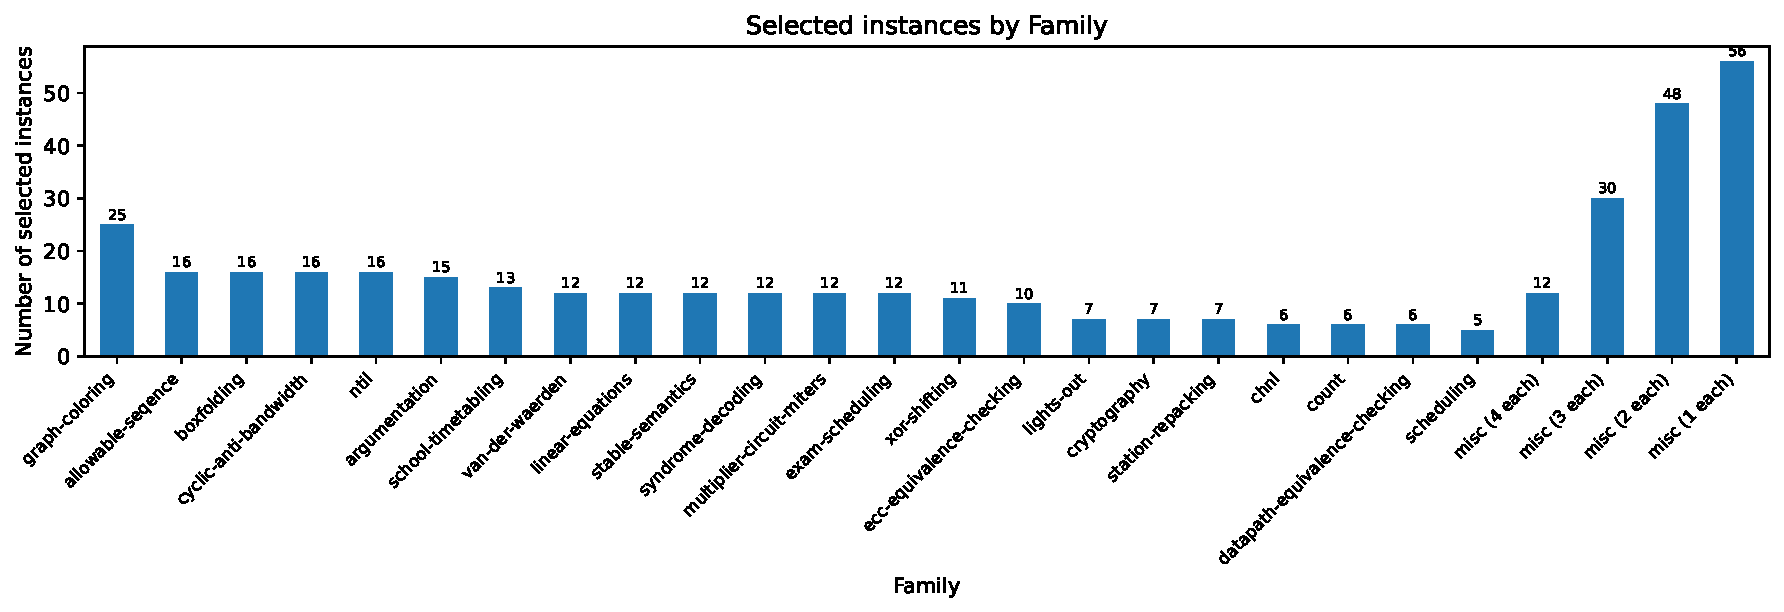
\includegraphics[width=\textwidth]{hist_family.pdf}
\caption{Number of selected instances per instance family.}
\label{fig:hist-family}
\end{figure*}

\begin{figure*}
\centering
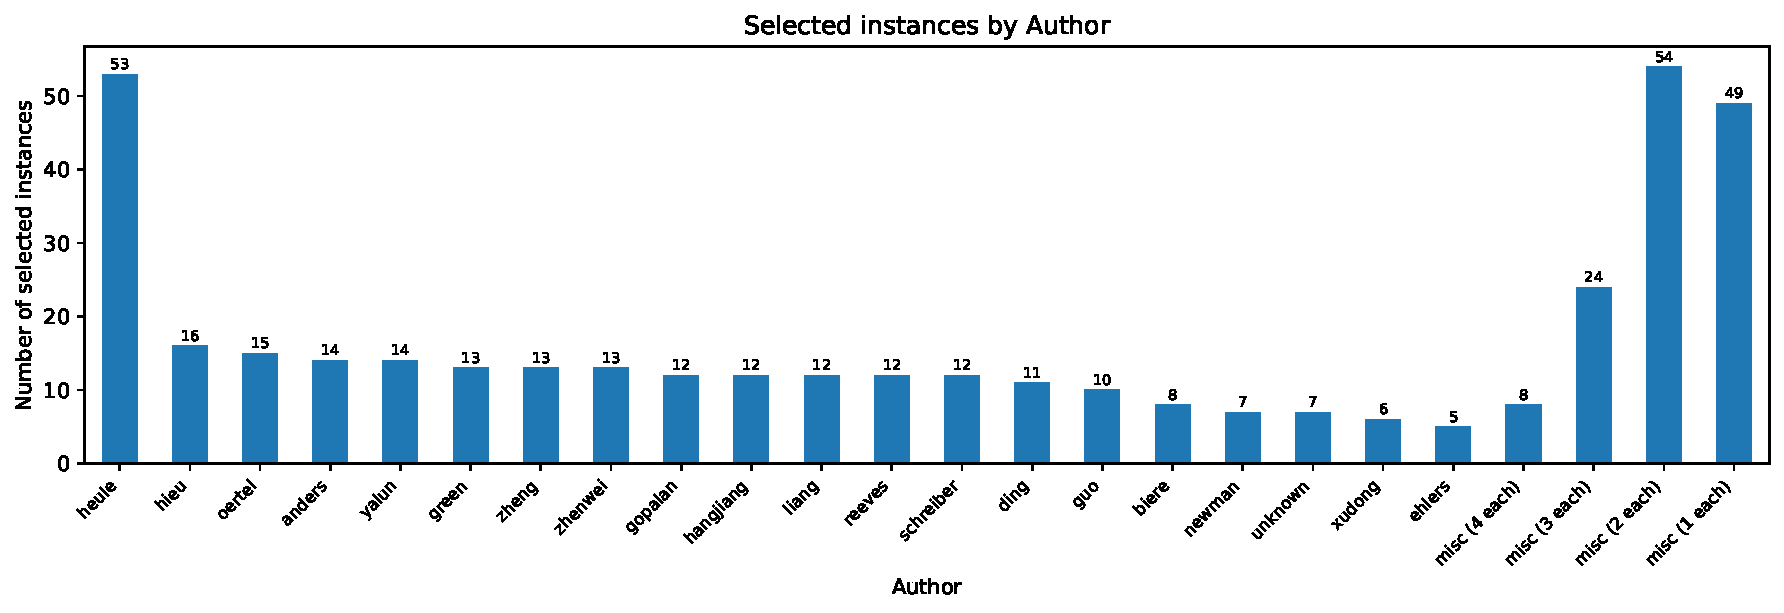
\includegraphics[width=\textwidth]{hist_author.pdf}
\caption{Number of selected instances per author.}
\label{fig:hist-author}
\end{figure*}


\section{Discussion}\label{sec:discussion}

% also point to dagstuhl and the FLoC workshop
% Discussion: time limit, criteria, hardness filter minisat
% discussion: reevaluate recency as smallest value of formula is smaller than 0.2, the baseline weight.

The 2026 benchmark set comprises 400 instances, evenly split between 146 satisfiable and 146 unsatisfiable instances and complemented by 108 instances of a priori unknown status.
Of these, 233 stem from new submissions and 167 from the historical pool in the GBD, so that the set reflects the current interests of the community while preserving comparability with previous competitions.
The large fraction of unknown instances is intentional and ensures that the set retains a sufficient number of genuinely challenging instances.

In our view, making the selection script publicly available well before the submission deadline was the most consequential step of this edition.
It let participants understand exactly how their submissions would be treated and inspect the weighting and balancing criteria in advance.
Together with the switch to the more precise IsoHash2 identifier and the deterministic revision of the script, the selection is now reproducible and auditable end to end.

The selection procedure introduces several deliberate biases.
The \emph{hardness} uses Minisat as its reference solver, the SAT/UNSAT \emph{balancing} relies on satisfiability and hardness statuses established by solvers from previous competitions, the \emph{novelty} weights favor newer instances, and the \emph{diversity} weights favor less-represented authors and families.
Including historical instances may benefit solvers that have been optimized for them.
Conversely, the strong emphasis on previously unseen submissions rewards robustness to new challenges and gives the actively submitting community greater influence over the composition of the benchmark set.
Excluding randomly generated instances prioritizes crafted and application instances, which are more likely to reflect problems of practical or scientific interest.
We consider these biases reasonable and well justified in the context of the competition, while recognizing that they represent design choices rather than uniquely correct decisions and may therefore be revisited in future editions.

\begin{thebibliography}{00}
    \bibitem{minisat} N. Eén and N. Sörensson, ``An Extensible SAT-solver'', in Selected Revised Papers of the Sixth International Conference on Theory and Applications of Satisfiability Testing, 2003, \url{https://doi.org/10.1007/978-3-540-24605-3_37}
    \bibitem{sc2017proc} Proceedings of SAT Competition 2017: Solver and Benchmark Descriptions, T. Balyo, M. J. H. Heule, and M. Järvisalo (editors), \url{http://hdl.handle.net/10138/231848}
    \bibitem{sc2020aij} N. Froleyks, M. J. H. Heule, A. Iser, M. Järvisalo, and M. Suda, ``The SAT Competition 2020'', Artificial Intelligence, vol. 301, 2021, \url{https://doi.org/10.1016/j.artint.2021.103572}
    \bibitem{sc2022proc} Proceedings of SAT Competition 2022: Solver and Benchmark Descriptions, T. Balyo, M. J. H. Heule, A. Iser, M. Järvisalo, and M. Suda (editors), \url{http://hdl.handle.net/10138/359079}
    \bibitem{bench23report} A. Iser, ``Benchmark Compilation for SAT Competition 2023.'', in Proceedings of SAT Competition 2023: Solver, Benchmark and Proof Checker Descriptions, \url{http://hdl.handle.net/10138/563824}
    \bibitem{gbdsatpaper} A. Iser and C. Jabs, ``Global Benchmark Database'', in Proceedings of SAT 2024, \url{https://doi.org/10.4230/LIPIcs.SAT.2024.18}
    \bibitem{sc2026web} K. Fazekas, M. J. H. Heule, and A. Iser, Webpage of SAT Competition 2026, \url{https://satcompetition.github.io/2026/}
    \bibitem{isohash2} A. Iser and F. Gehm, ``Efficient Identification of Isomorphic SAT Instances'', in Proceedings of the International Conference on Theory and Applications of Satisfiability Testing (SAT), 2026, \url{https://doi.org/10.4230/LIPIcs.SAT.2026.35}
\end{thebibliography}


\end{document}